\documentclass{article}
\usepackage{amsmath}
\usepackage{graphicx}
\usepackage[table,xcdraw]{xcolor}
\usepackage{hyperref}
\usepackage{subcaption}
\usepackage{soul}
\usepackage{multirow}
\title{CSE 200: Technical Writing and Presentation}
\author{Online 1}
\date{24 September, 2024}

\begin{document}

\maketitle

\section{Text Formatting}
You can format text in multiple ways in LaTeX:
\begin{itemize}
    \item \textbf{Bold text}: For emphasizing important words.
    \item \textit{Italicized text}: Commonly used for names of books, papers, or emphasis.
    \item \underline{Underlined text}: Useful for highlighting.
    \item \textcolor{red}{Colored text}: Color can be applied to any text for emphasis or visual interest.
    \item \st{Strikethrough text}: Used to indicate deletion or change.
\end{itemize}


\section{Nested Lists with Different Bullets and Numbering}
Below is an example of nested lists with different bullet and numbering styles:
\begin{enumerate}
    \item First level
    \begin{enumerate}
        \item Second level with letters
        \begin{enumerate}
            \item[i.] Third level with Roman numerals
            \begin{enumerate}
                 \item[$\bullet$] Fourth level with bullet points
                  \begin{enumerate}
                     \item[--] Fifth level with dashes
                 \end{enumerate}
            \end{enumerate}
        \end{enumerate}
        \item Another first level item
    \end{enumerate}
\end{enumerate}


\section{Equations}
\section*{\textbf{Equation 1}}
$$
    w(a) = 
        \begin{cases} 
        (\Pi_{(u,v)\in p_a} w_{(u,v)})^-1 & \text{if } x_1 \leq x < x_2 \\
        1    & \text{otherwise} 
\end{cases}
$$

\section*{\textbf{Equation 2}}
\[\vec{q}_x = \frac{2g_x}{k-1}\vec{b}_n, \quad \vec{q}_y = \frac{2g_y}{m-1}\vec{v}_n, \quad \vec{p}_{1m} = \vec{t}_n d - g_x\vec{b}_n - q_y\vec{v}_n\]

\section*{\textbf{Equation 3}}
\[S(n,k) = \frac{1}{k!}\sum_{i=0}^k (-1)^{k-i}\binom{k}{i}i^n = \sum_{i=0}^k \frac{(-1)^{k-i} i^n}{(k-i)!i!} \quad (3)\]

\section*{ Equation 4}
\[F_c(x,y) = \begin{cases} 
\frac{\partial^2 x^3y^x}{\partial x^2} + \frac{\partial^2\Gamma(x)\log(\tan y)}{\partial x\partial y} & \text{if x,y are real numbers} \\[10pt]
\displaystyle\lim_{z \to e^{x^{2y}}}\sqrt{Z + \frac{a}{\sqrt{z + \frac{1}{z+...}}}} & \text{otherwise}
\end{cases}\]

\section*{ Equation 5}
\[e^{i\theta} = \cos \theta + i \sin \theta\]

\text{if we put } \theta = \frac{\pi}{2} \text{ in equation 5, we get the following:}

\[e^{i\frac{\pi}{2}} = \cos \frac{\pi}{2} + i \sin \frac{\pi}{2}\]
\[= 0 + i.1\]
\[= i\]


\section{Table}
\begin{tabular}{|c|c|c|c|}
\hline
Row Header & \multicolumn{2}{c|}{Multi column Header} & Single Column \\
\cline{2-3}
& Col 1 & Col 2 & \\
\hline
Row 1 & \multicolumn{2}{c|}{1.5} & Info 1 \\
\cline{2-3}
& 1.4 & 1.9 & \\
\hline
Row 2 & \multirow{2}{*}{1.0} & 1.5 & Info 3 \\
\cline{3-3}
& & 1.4 & \\
\hline
\end{tabular}

\pagebreak


\section{Subfigures}
You can use subfigures to include multiple images within the same figure environment. For example, see figure \ref{fig:subfigures}.

\begin{figure}[h]
    \centering
    \begin{subfigure}[b]{0.4\textwidth}
        
\includegraphics[width=\textwidth]{CSE_BUET.png}
        \caption{Image 1}
    \end{subfigure}
    \hfill
    \begin{subfigure}[b]{0.55\textwidth}
        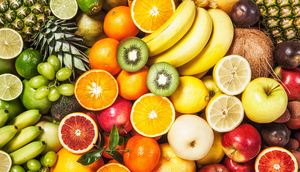
\includegraphics[width=\textwidth]{Fruits.png}
        \caption{Image 2}
    \end{subfigure}
    
    \vspace{1em}
    
    \begin{subfigure}[b]{0.55\textwidth}
        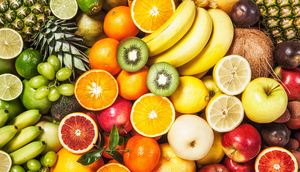
\includegraphics[width=\textwidth]{Fruits.png}
        \caption{Image 3}
    \end{subfigure}
    \hfill
    \begin{subfigure}[b]{0.4\textwidth}
        
\includegraphics[width=\textwidth]{CSE_BUET.png}
        \caption{Image 4}
    \end{subfigure}
    \caption{Four Images}
    \label{fig:subfigures}
\end{figure}


\section{Referencing}
A very popular method of phylogenetic tree estimation is ASTRAL \cite{Mirarab2014}. Another equally or better-performing method is wQFM \cite{Mahbub2021}, developed in our department.

\bibliographystyle{plain}
% \bibliography{references}

\begin{thebibliography}{9}

    \bibitem{Mirarab2014} Mirarab, S. et al. (Aug. 2014). ``ASTRAL: genome-scale coalescent-based species tree estimation''. In: \textit{Bioinformatics} 30.17, pp. 541--548. \textsc{issn}: 1367-4803. \textsc{doi}: 10.1093/bioinformatics/btu462. \textsc{url}: \url{https://doi.org/10.1093/bioinformatics/btu462}.

    \bibitem{Mahbub2021} Mahbub, Mahin et al. (June 2021). ``wQFM: highly accurate genome-scale species tree estimation from weighted quartets''. In: \textit{Bioinformatics} 37.21, pp. 3734--3743. \textsc{issn}: 1367-4803. \textsc{doi}: 10.1093/bioinformatics/btab428. \textsc{url}: \url{https://doi.org/10.1093/bioinformatics/btab428}.
\end{thebibliography}

\end{document}


